\section{Wstęp}

\subsection{Testowa baza danych}
Aby przedstawić techniki optymalizacji zawarte w pracy na rzeczywistych przykładach, wykorzystałem bazę danych udostępnioną przez portal \textit{stackoverflow.com}. Baza zawiera w granicach 50 Gb danych zebranych w latach 2008-2013. Archiwum po zaimportowaniu do serwera MySQL nie zawiera kluczy głównych, kluczy obcych, indeksów.
Początkowy schemat bazy danych jest przedstawiony na rysunku 1.
\begin{figure}
    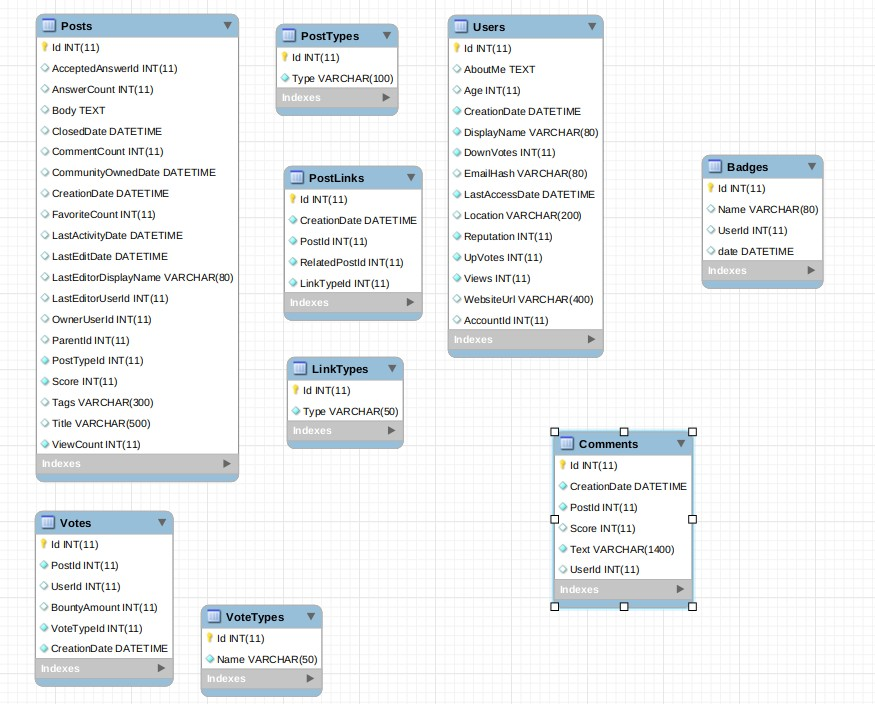
\includegraphics[scale =0.5]{schemat-baza-stackoverflow.jpg} 
    \caption{Schemat bazy danych stackoverflow}
\end{figure}
